\documentclass[12pt]{article}
\usepackage[utf8]{inputenc}
\usepackage[T1]{fontenc}
\usepackage{lmodern}
\usepackage{graphicx}
\usepackage{subcaption}
\usepackage[svgnames]{xcolor}
\usepackage[a4paper,bindingoffset=0.2in,%
            left=0.5in,right=0.5in,top=0.5in,bottom=1in,%
            footskip=.25in]{geometry}
\pagenumbering{gobble}
\usepackage[colorlinks=true, linkcolor=Black, urlcolor=Blue]{hyperref}

\begin{document}
\title{Sprawozdania z zajęć z prototypowania}
\author{Sebastian Michoń 136770, Mateusz Wankowski 136823,\\ Piotr Król XXXXXX, Maciej Leszczyk 136759}
\date{\vspace{-3ex}}
\maketitle

\section{Idee, koncepcje, motywacje}
Ideą naszego prototypu było stworzenie aplikacji wspomagania systemu kolejkowego, podobnej do politechnicznego Zintegrowanego Centrum Obsługi. Uznaliśmy, że aplikacja politechniczna jest wysoce niedoskonała, skłoniło nas to do pokazania światu nowej, po wielokroć wspanialszej wersji tego systemu, z liczbą opcji, o których paniom z dziekanatu się nie śniło. Nasz aplikacja powinna mieć charakter mobilny, co umożliwi korzystanie z niej poza politechniką.

\section{I etap prototypowania}
\subsection {Indywidualne pomysły}
\begin {enumerate}
	\item Pierwsza koncepcja indywidualna Piotra to możliwość stwierdzenia przy pobraniu biletu, o której dana osoba wchodzi do dziekanatu i czy zgadza się na przesuwanie jej w kolejce na wcześniejszy termin: uznaliśmy, że jeśli osoba ma termin wizyty o kilka godzin późniejszy niż termin pobrania biletu, może chcieć na przykład zjeść obiad w trakcie czasu oczekiwania - natomiast jeśli i tak czeka w poczekalni, może się zgodzić na przesuwanie jej na jak najwcześniejszy termin jeśli jakaś wizyta potrwa krócej niż oczekiwano albo ktoś zrezygnuje z wizyty.
	
	\item Mateusz zauważył, że jeśli ktoś woli czekać w kolejce, to zapewne nie ma niczego ciekawszego z jego perspektywy niż wchodzenie w interakcję z innymi ludźmi - a co za tym idzie, dobrze by było, gdyby nasza aplikacja była wyposażona w substytut messengera przeznaczony dla ludzi partycypujących w naszym systemie kolejkowym. Funkcjonalność ta uwzględnia możliwość dołączenia do czatu grupowego dla wszystkich osób będących w kolejce, oraz wysyłania wiadomości prywatnych. Wiadomości prywatne można jednak wysyłać tylko do osób które zgodziły się na otrzymywanie wiadomości od innych użytkowników zaznaczając odpowiedniego checkboxa.
	
	\item Pomysł Macieja polegał na możliwości przeglądania osób znajdujących się razem z nami w kolejce. Po zalogowaniu się i dołączeniu do poczekalni użytkownik widzi swoje informacje personalne wraz ze zdjęciem, numerkiem w kolejce oraz szacowanym czasem oczekiwania. Oprócz tego interfejs wyposażony jest w guziki next i previous dzięki którym użytkownik może dostrzec analogiczne informacje o innych uczestnikach z kolejki. Idea ta wydawała się dziwna i niepotrzebna, jednak połączyliśmy ją z poprzednim pomysłem i dzięki temu możemy wchodzić w konwersację prywatną z innymi użytkownika korzystając właśnie z tego interfejsu.	
	
	\item Sebastian spostrzegł, że dobrze by było, gdyby osoba zalogowana do systemu miała możliwość obejrzenia swojej historii wizyt w dziekanacie - żeby przypomnieć sobie, z kim ostatnio prowadziła konwersację na przykład po to, żeby później móc dostarczyć mailem zaległą informację, której nie była w stanie podać w trakcie wizyty.

\end {enumerate}

\subsection {Co wspólne, co różne}
Wspólną cechą wszystkich projektów były 2 funkcjonalności różne od głównej - możliwość zalogowania się do systemu albo anonimowego użytkowania aplikacji, a także szacowanie czasu pozostałego do wizyty. Różne indywidua wysnuwały jednakże różne wnioski z tych funkcjonalności - jedni opierali o nie funkcjonalność chatu, inni historię i zgodę na przesuwanie w kolejce. Poza tymi 2 kwestiami wszystko inne było różne.

\subsection{Co okazało się dobrym pomysłem, co nie}
\begin {enumerate}
	\item Chat okazał się niezgorszym pomysłem, uznaliśmy, że wielu jest ludzi pragnących w trakcie oczekiwania w kolejce prowadzić konwersację z innymi personami. 
	
	\item Możliwość stwierdzenia, czy osoba woli być przesuwana także jest opcją, która jest z naszej perspektywy bardzo zasadna - przy długim czasie oczekiwania danie użytkownikowi możliwości przyjścia o konkretnej godzinie pozwala mu spożytkować swój czas na inne aktywności niż stanie w kolejce.
	
	\item Historia poprzednich wizyt okazała się przeciętnym pomysłem, niektórzy uważają, że jej jedynym zastosowaniem jest sprawdzenie, ile czasu swojego życia zmarnowało się w niezrównanym królestwie biurokracji zwanym dziekanatem, niemniej jednak może stanowić niemałą pomoc dla ludzi roztargnionych i nierozgarniętych, dlatego zdecydowaliśmy się ją uwzględnić w II etapie projektowania apikacji.
	
\end {enumerate}

\section {Wnioski z II etapu projektowania aplikacji}
\subsection {Które pomysły zostały zrealizowane, które nie?}

Wszystkie indywidualne pomysły zostały zaimplementowane w naszej aplikacji, jednak część z nich w inny sposób niż wyobrażał to sobie autor - w pełni zrealizowaline zostały koncepcje historii i zgody na przesuwanie w kolejce, z kolei chat został połączony z możliwością przeglądania użytkowników w kolejce.

\subsection{Które pomysły okazały się trafione, które nie według osób spoza grupy?}
\begin{enumerate}
	\item Trafionym pomysłem okazał się chat razem z możliwością przeglądania innych osób znajdujących się w kolejce - ludzie spoza grupy byli bardzo skorzy do korzystania z tej funkcjonalności aplikacji, może nawet bardziej niż z jej głównej funcjonalności.
	\item Prosta funkcjonalność zgody na przesuwanie w kolejce zgodnie z oczekiwaniami nie wzbudzała wielkiego zainteresowania, natomiast różne osoby wybierały albo nie wybierały tą opcję - a co za tym idzie, była zauważana i spełniała swoje zadanie.
	\item Historia wzbudzała kontrowersje - jedni twierdzili, że jest absolutnie zbędna, inni, że może być bardzo pomocna w dostarczaniu zaległych informacji.
\end{enumerate}


\clearpage


\begin{figure}[h!]
	\section {Aplikacja w akcji}
	\subsection{Wygląd całej aplikacji}
	\centering
	\begin{subfigure}[b]{1\linewidth}
		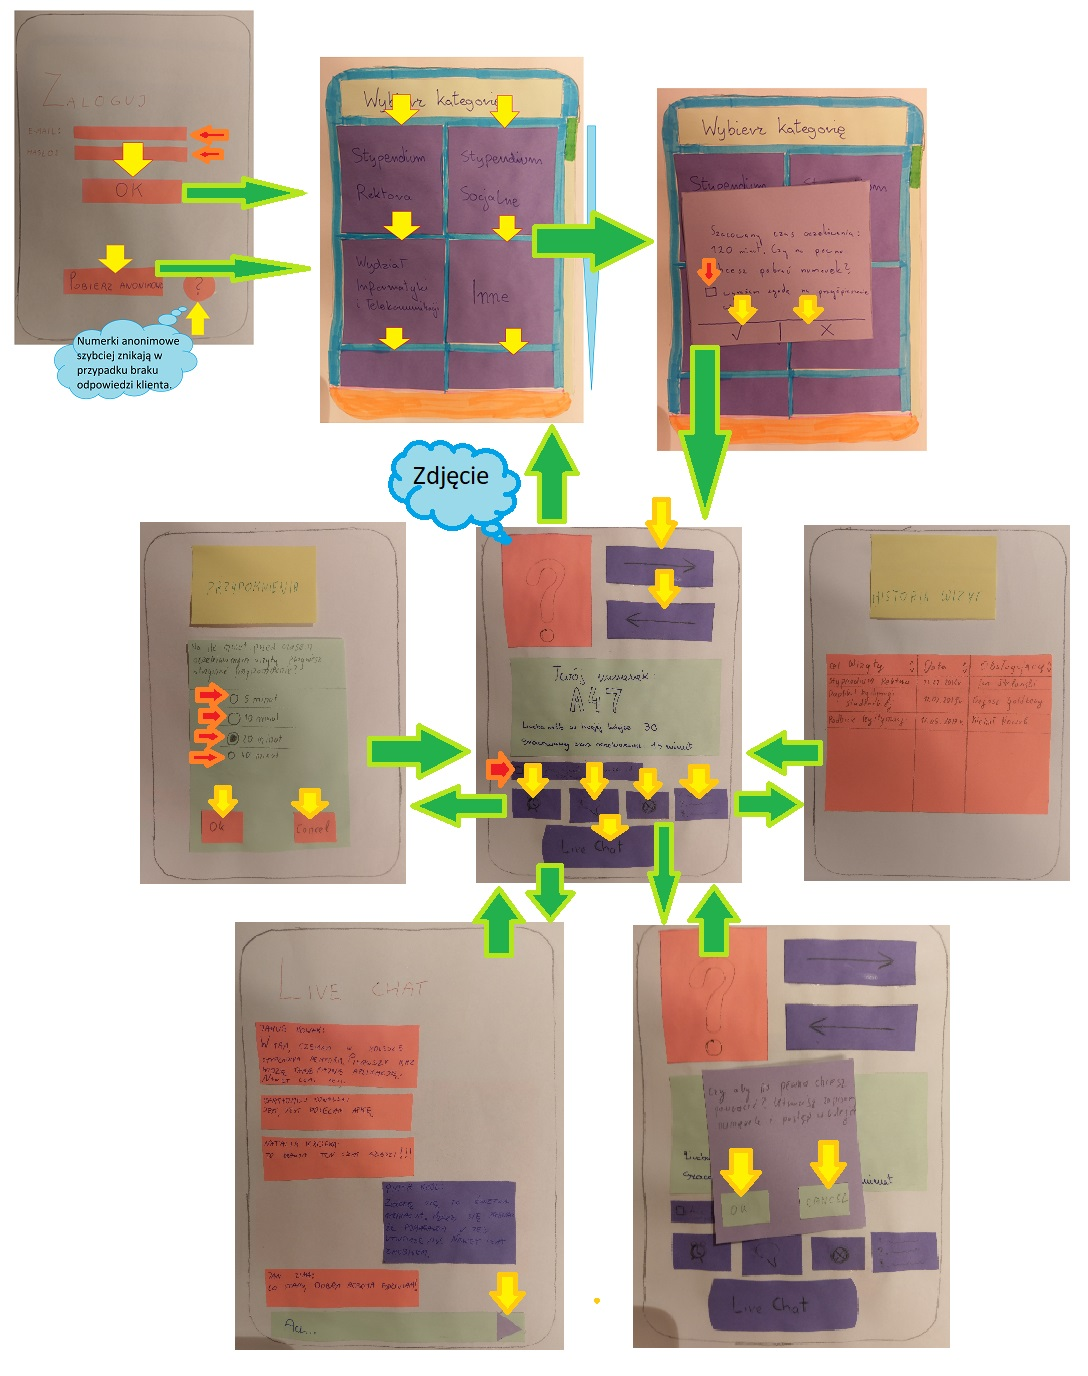
\includegraphics[width=\linewidth]{zdj/mozaika.jpg}
		\caption{\underline{Podpis}}
	\end{subfigure}
	\label{fig:nuty}
	\caption{Nawigacja}
\end{figure}

\clearpage
\subsection{Działanie aplikacji:}
\begin {enumerate}
	\item Pierwszym ekranem, na który natrafi użytkownik korzystający z aplikacji jest ekran "zaloguj". Są na nim 2 pola tekstowe na email i hasło do politechnicznego ekonta, a także przyciski: "zaloguj", "pobierz anonimowo" i "?". Przycisk "?" podaje informację o szybszym znikaniu numerków anonimowych. Jeśli użytkownik poda złe hasło/login, po kliknięciu przycisku "OK" wyświetli się czerwony komunikat pod przyciskiem "OK": "Niepoprawne dane logowania". Oczywiście "Pobierz anonimowo" pozwala przejść do następnego okna bez logowania.
	
	\item Drugi ekran to ekran wyboru kategorii. Są tam takie opcje, jak: "Stypendium rektora", "Leigtymacja studencka", "Stypendium socjalne", a także kategoria specjalna, nie powodująca pobrania numerka: "Historia".
	
	\item Po wybraniu kategorii różnej od historii pokazuje się komunikat: "Szacowany czas oczekiwania: ${x}$ minut. Czy na pewno chcesz pobrać numerek? Niżej jest checkbox "Wyrażam zgodę na przyspieszenie wizyty". Zaznaczenie checkboxa powoduje, że czas oczekiwania może się zmniejszyć. Użytkownik może kliknąć "v"(wziąć numerek) lub "x" (nie wziąć numerka).
	
	\item Po wzięciu numerka ukazuje się ekran główny. Na nim jest zdjęcie użytkownika, strzałki w lewo i prawo\underline{WYPEŁNIĆ - CO TO DAJE, ZNACZENIE W KONTEKŚCIE LIVE CHATA}, a także wyśrodkowana informacja o numerze użytkownika, szacowanym pozostałym czasie oczekiwania i liczbie osób w kolejce przed nim. Poniżej przyciski - przycisk ze znakiem budzika prowadzi do ekranu przypomnień, przycisk ze znakiem listy numerowanej do historii, przycisk ze znakiem x-a w kółku do wyjścia z aplikacji,\underline{WYPEŁNIĆ - CO ROBI ZNAK CHMURKI}, przycisk z napisem "Live Chat" prowadzi do czata grupowego. Co istotne, kliknięcie przycisku powrotu w telefonie prowadzi do komunikatu z ostrzeżeniem "Czy na pewno chcesz powrócić? Stracisz numerek i postęp w kolejce".
	
	\item Ekran historii przedstawia tabelę z ceem wizyty, datą i nazwiskiem człowieka, u którego rozwiązywano daną kwestię. Dane można sortować dla wygody przyciskami "\^{}" i "v" przy nagłówku kolumny. Kliknięcie powrotu na telefonie prowadzi do okna głównego albo okna kategorii, zależnie od poprzedniego okna.
	
	\item Ekran przypomnień pozwala na ustawienie przypomnienia na $x$ minut przed wizytą, gdzie $x\in\{5, 10, 20, 40\}$. Przycisk "OK" ustawia przypomnienie, przycisk "Cancel" nie ustawia przypomnienia i usuwa ustawione wcześniej przypomnienie przez tą aplikację, jeśli takie było. Powrót na telefonie po prostu wraca do poprzedniego ekranu (ekran główny)
	
	\item \underline{WYPEŁNIĆ - JAK DZIAŁA LIVECHAT}
	
\end{enumerate}


\clearpage
\subsection{Przykaładowe scenariusze}
(kursywą oznaczam zalety aplikacji pokazane w scenariuszu i elementy ewaluacji heurystcznej)
\begin {enumerate}
	\item Użytkownik A postanawia złożyć wniosek o stypendium rektora. Loguje się do systemu, następnie klika na kategorię "Stypendium Rektora". Dostaję informację - szacowany czas oczekiwania to 150 minut; uznaje, że lepiej spożytkuje ten czas idąc do restauracji i spożywając tam obiad niż czekając w poczekalni, dlatego nie klika na checkbox (Wyrażam zgodę na przyspieszanie wizyty), ale klika od razu na przycisk v. Oczom naszego delikwenta ukazuje się numerek, a także pozostały czas oczekiwania. Użytkownik uznaje, że dobrze byłoby ustawić sobie przypomnienie, aby nie zapomnieć o wizycie; dlatego klika na znaczek budzika, następnie dotyka checkboxa przy napisie "20 minut" i klika OK, przechodząc tym samym do ekranu głównego. Użytkownik po otrzymaniu przypomnienia ok. 130 minut później przybywa do dziekanatu, rozwiązuje swój problem i zamyka aplikację.
	
	\textit{Aplikacja nie komunikuje zbędnych informacji - użytkownik nie musi analizować rozległych okien dialogowych, które są w dużej mierze bezużyteczne, jedynie bardzo mały zbiór informacji niezbędnych do uzyskania oczekiwanego przez niego efektu, a co za tym idzie, jeśli jakiś komunikat aplikacji jest użyteczny to prawie na pewno zostanie spostrzeżony przez użytkownika.}\\
	
	
	\item Użytkownik B postanawia wyrobić duplikat legitymacji studenckiej. Loguje się zatem do systemu i klika na opcję "Legitymacja Studencka". Otzymuje informację o tym, że szacowany czas oczekiwania to 70 minut. Uznaje, że spędzi ten czas w poczekalni, dlatego zgadza się na przesuwanie wizyty na wcześniejszy termin. Użytkownik następnie klika przypadkowo na znak powrotu w telefonie, widząc chwilę później komunikat "Czy na pewno chcesz powrócić? stracisz numerek i postęp w kolejce" klika przycisk cancel, ponieważ nie taka jest jego wola. Następnie klika opcję "Live Chat", bo nie ma co robić, i rozpoczyna konwersację z innymi użytkownikami tej aplikacji. Gdy nadchodzi czas na obsługę jego numerka wchodzi do dziekanatu, rozwiązuje swój problem i zamyka aplikację.
	
	\textit{Komunikaty ostrzegawcze są przedstawione w prostym języku i jednoznacznie wskazują na konsekwencję danego działania; istnieje wyjście ratunkowe z niechcianej sytuacji.}\\
	
	\item Użytkownik C postanawia skorzystać anonimowo z aplikacji po przeczytaniu informacji "Numerki anonimowe szybciej znikają w przypadku braku odpowiedzi klienta" zauważonej po kliknięciu w przycisk "?". Wybiera opcję "Stypendium socjalne", otrzymuje komunikat "Szacowany czas oczekiwania: 13726 miunt. Czy na pewno chcesz pobrać numerek?". Uznaje, że nie zamierza czekać 229 godzin w kolejce, dlatego klika "x" i zamyka aplikację.
	
	\textit{Istnieje pomoc dla użytkownika zagubionego w gąszczu opcji; istnieje wyjście ratunkowe z niechcianej sytuacji.}\\
	
	
	\item Użytkownik D chce jedynie dosłać przez maila informację dla osoby, która poprzednio go obsługiwała, dlatego po zalogowaniu się wybiera kategorię historia(do użycia której nie potrzebuje numerka). Sprawdza, kto ostatnio go obsługiwał w dziekanacie, aby później wysłać tej osobie maila, następnie zamyka aplikację.\\
	
	\textit{Wymienione sytuacje całościowo pokazują kilka innych wartościowych heurystyk aplikacji: interfejs użytkownika daje wiedzę o tym, co się dzieje w systemie, poza ekranem głownym użytkownik zawsze widzi na szczycie aplikacji nazwę ekranu,na którym się znajduje. Wszystkie opcje są widoczne z poziomu ekranu głównego; komunikaty są jednoznaczne, nie dają dużej przestrzeni na swobodne interpretacje.}

\end{enumerate}

\end{document}
